\documentclass[11pt,a4paper,headinclude,footinclude,DIV16,normalheadings]{scrreprt}
\usepackage[automark]{scrpage2}
\usepackage[ansinew]{inputenc}
%\usepackage{german}
%\usepackage{bibgerm}
\usepackage{amsmath}
\usepackage{amsfonts}
\usepackage{theorem}
\usepackage{color}
\usepackage{listings}
\lstset{language=C++, basicstyle=\ttfamily, 
  keywordstyle=\color{black}\bfseries, tabsize=4,
  stringstyle=\ttfamily, commentstyle=\it, extendedchars=true}
\usepackage{hyperref}
\usepackage{psfrag}
\usepackage{makeidx}

\newif\ifpdf
\ifx\pdfoutput\undefined
\pdffalse % we are not running PDFLaTeX
\else
\pdfoutput=1 % we are running PDFLaTeX
\pdftrue
\fi

\ifpdf
\usepackage[pdftex]{graphicx}
\else
\usepackage{graphicx}
\fi

\ifpdf
\DeclareGraphicsExtensions{.pdf, .jpg, .tif}
\else
\DeclareGraphicsExtensions{.eps, .jpg}
\fi

\newcommand{\C}{\mathbb{C}}
\newcommand{\R}{\mathbb{R}}
\newcommand{\N}{\mathbb{N}}
\newcommand{\Z}{\mathbb{Z}}
\newcommand{\Q}{\mathbb{Q}}
\newcommand{\Dune}{{\sf\bfseries DUNE}}

%The theorems
\theorembodyfont{\upshape}
\theoremheaderfont{\sffamily\bfseries}
\newtheorem{exc}{Excercise}[chapter]
\newtheorem{rem}[exc]{Remark}
\newtheorem{lst}{Listing}
\newtheorem{warn}[exc]{Warning}

\pagestyle{scrheadings}

\title{The Distributed and Unified Numerics Environment (DUNE) Grid
  Interface HOWTO}

\author{Peter Bastian$^\ast$ \and 
Markus Blatt$^\ast$ \and
Andreas Dedner$^\dagger$ \and 
Christian Engwer$^\ast$ \and  
Robert Kl�fkorn$^\dagger$ \and 
Mario Ohlberger$^\dagger$ \and  
Oliver Sander$^\ddagger$}

\date{\today}

\publishers{%
\vspace{10mm}
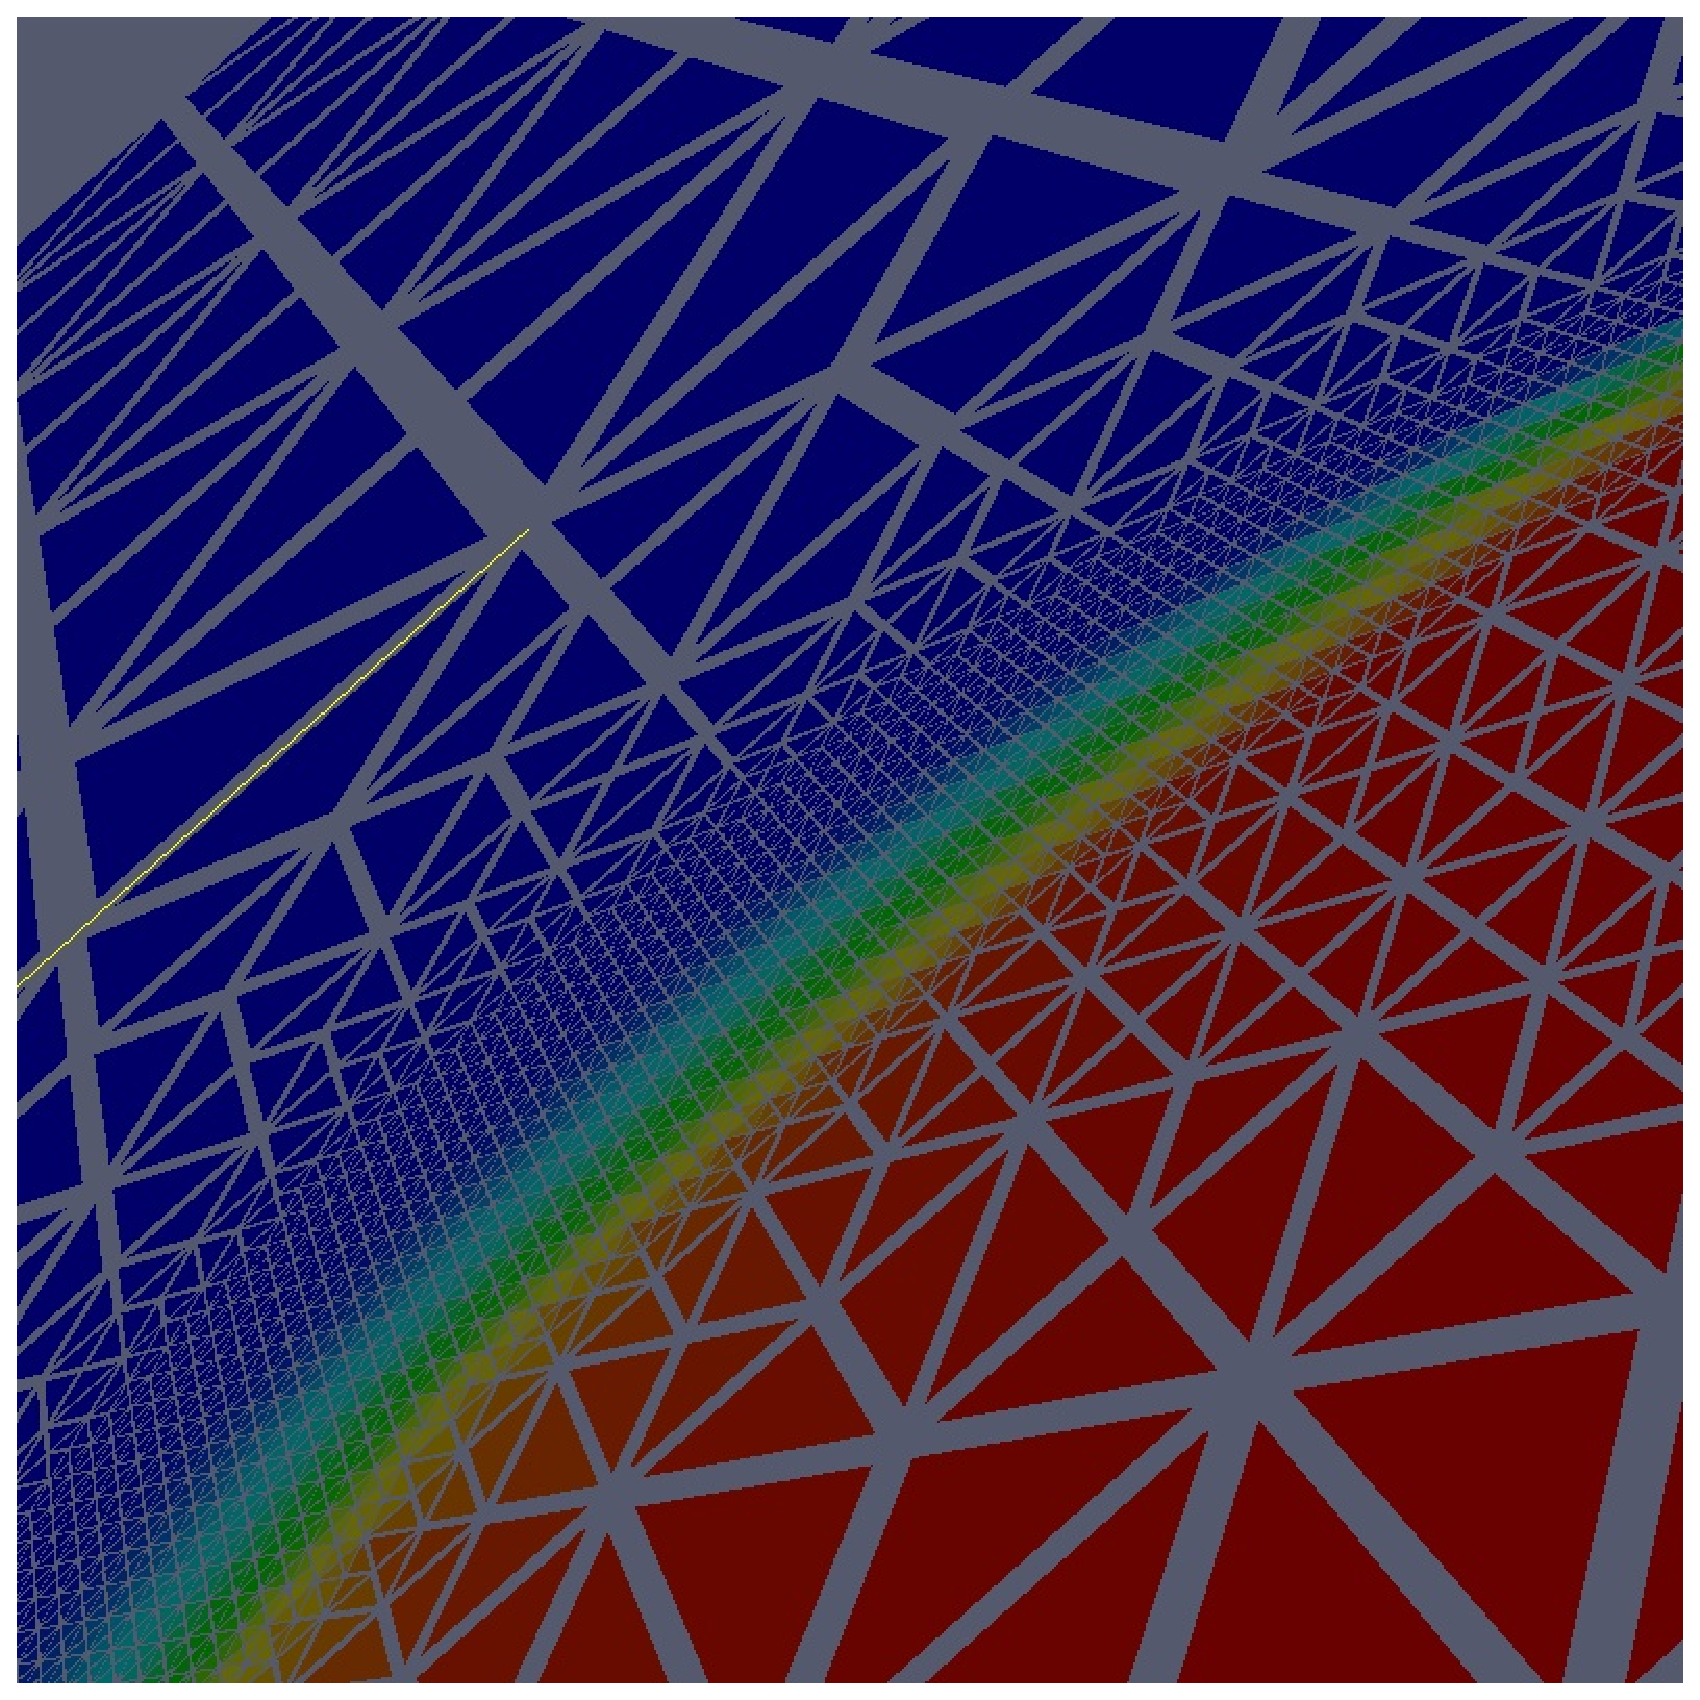
\includegraphics[width=0.32\textwidth]{EPS/alberta2d-view2.eps}\hfill
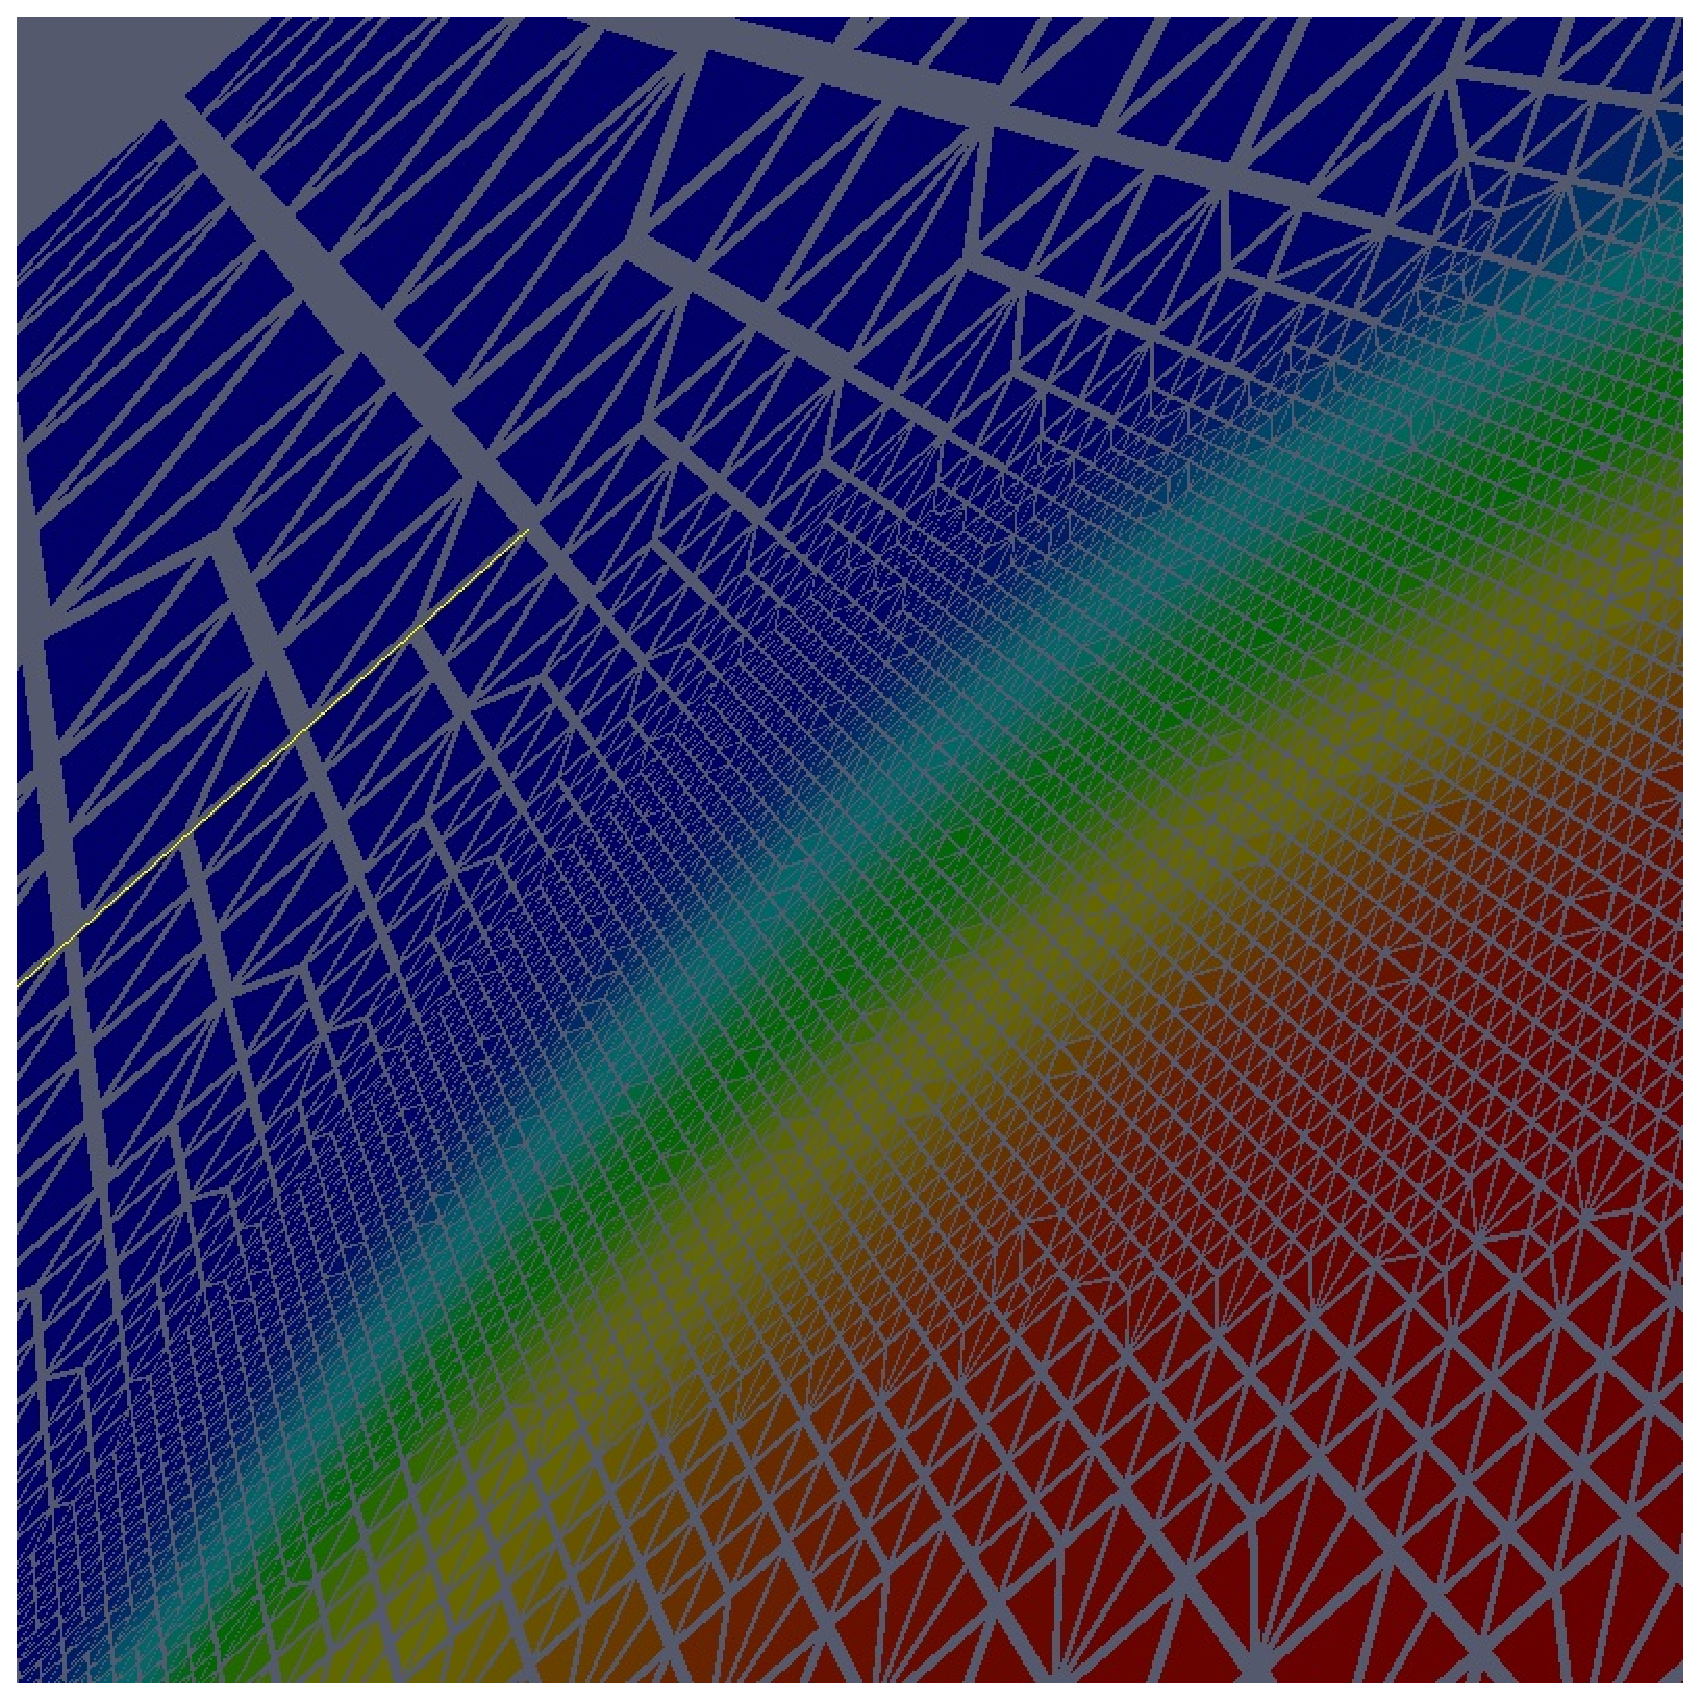
\includegraphics[width=0.32\textwidth]{EPS/ug2dtri-view2.eps}\hfill
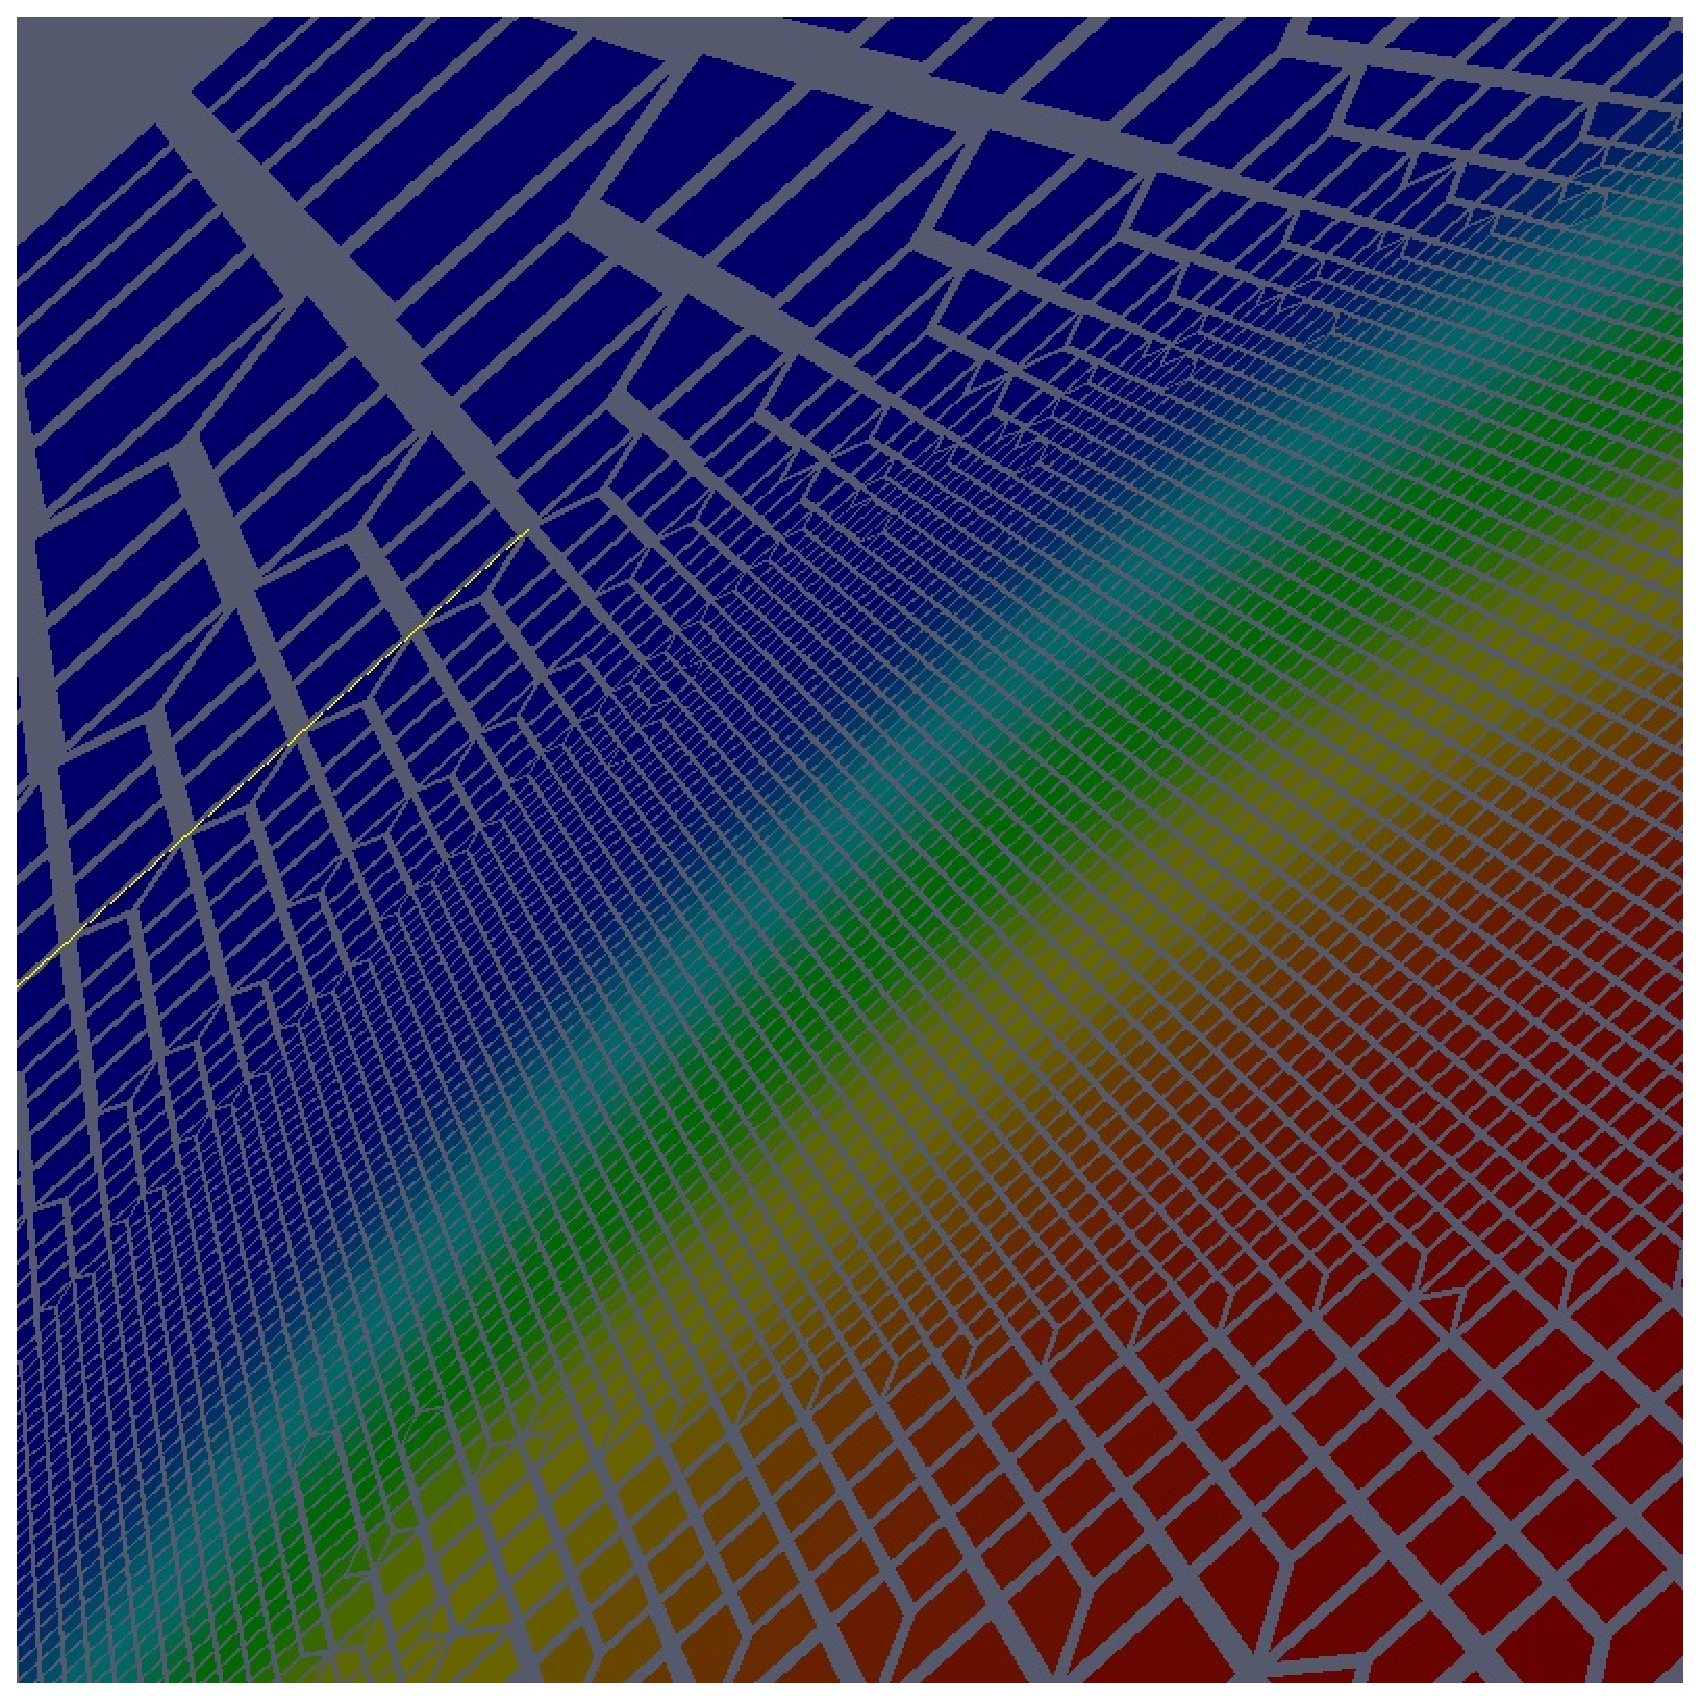
\includegraphics[width=0.32\textwidth]{EPS/ug2dquad-view2.eps}

\vspace{10mm}
{\normalsize $^\ast$Interdisziplin�res Zentrum f�r Wissenschaftliches Rechnen,
Universit�t Heidelberg,\\
Im Neuenheimer Feld 368, D-69120 Heidelberg, Germany}\\
%
\bigskip
{\normalsize $^\dagger$Abteilung f�r Angewandte Mathematik, Universit�t Freiburg,\\
Hermann-Herder-Str.~10, D-79104 Freiburg, Germany}\\
%
\bigskip
{\normalsize $^\ddagger$Institut f�r Mathematik II,\\ Freie Universit�t Berlin,
Arnimallee 2-6, D-14195 Berlin, Germany}\\
%
\bigskip
{\normalsize \texttt{http://hal.iwr.uni-heidelberg.de/dune/index.html}}\\
}

\makeindex

\begin{document}

\maketitle

\begin{abstract}
This document gives an introduction to the Distributed and Unified
Numerics Environment (\Dune). \Dune\ is a template library for the
numerical solution of partial differential equations. It is based on
the follwing principles: i) Seperation of data structures and
algorithms by abstract interfaces, ii) Efficient implementation of these
interfaces using generic programming techniques (templates) in C++ and
iii) Reuse of existing finite element packages with a large body of
functionality. This introduction covers only the abstract grid interface
of \Dune\ which is currently the most developed part. However, part of
\Dune\ are also the Iterative Solver Template Library (ISTL, providing a
large variety of solvers for sparse linear systems) and a flexible class
hierarchy for finite element methods. These will be described in
subsequent documents. Now have fun!
\end{abstract}

\tableofcontents


%%%%%%%%%%%%%%%%%%%%%%%%%%%%%%%%%%%%%%%%%%%%%%%%%%%%%%%%%%%%%%%%%%%%%%%%%%%
%%%%%%%%%%%%%%%%%%%%%%%%%%%%%%%%%%%%%%%%%%%%%%%%%%%%%%%%%%%%%%%%%%%%%%%%%%%
\chapter{Introduction}
%%%%%%%%%%%%%%%%%%%%%%%%%%%%%%%%%%%%%%%%%%%%%%%%%%%%%%%%%%%%%%%%%%%%%%%%%%%
%%%%%%%%%%%%%%%%%%%%%%%%%%%%%%%%%%%%%%%%%%%%%%%%%%%%%%%%%%%%%%%%%%%%%%%%%%%

\section{What is Dune anyway?}

\Dune\ is a software framework for the numerical solution of partial
differential equations with grid-based methods. It is based on the
following main principles:
\begin{itemize}
\item \textit{Seperation of data structures and
algorithms by abstract interfaces.} This provides more functionality
with less code and also ensures maintainability and
extendability of the framework.
\item \textit{Efficient implementation of these
interfaces using generic programming techniques}. Static polymorphism
allows the compiler to do more optimizations, in particular function
inlining, which in turn allows the interface to have very small
functions (implemented by one or few machine instructions) without a
severe performance penalty. In essence the algorithms are parametrized
with a particular data structure and the interface is removed at
compile time. Thus the resulting code is as efficient as if it would
have been written for the special case.
\item \textit{Reuse of existing finite element packages with a large body of
functionality.} In particular the finite element codes UG, \cite{ug},
Alberta, \cite{Alberta}, and ALU3d, \cite{ALU3d}, have been
adapted to the \Dune\ framework. Thus, parallel and adaptive meshes with
multiple element types and refinement rules are available. All these
packages can be linked together in one executable.
\end{itemize}

The framework consists of a number of modules which are different
states of maturity. In particular these are:
\begin{itemize}
\item \textit{Grid interface.} This is the most mature module that is
  covered in this document. It defines nonconforming, hierarchically
  nested, multi-element-type, parallel grids in arbitrary space dimensions. 
\item \textit{Iterative Solver Template Library.} Provides generic
  sparse matrix/vector classes and a variety of solvers based on these
  classes. A special feature is the use of templates to exploit the
  recursive block structure of finite element matrices at compile
  time. Available solvers include Krylov methods, (block-) incomplete
  decompositions and aggregation-based algebraic multigrid.
\item \textit{Freiburg Finite Element Hierarchy.} A flexible class
  hierarchy for finite elements. Explicit cell-centered finite volume
  and discontinuous Galerkin methods for hyperbolic problems,
  e.~g.~transport in porous media and inviscid fluid flow have been implemented.
\item \textit{Heidelberg Finite Element Hierarchy.} Another flexible
  class hierarchy for finite elements. Standard and discontinuous
  Galerkin finite elements for elliptic problems, e.~g.~Laplacian,
  linear elasticity and Stokes have been implemented.
\item \textit{Input/Output.} Graphical output with several packages is
  available, e.~g.~file output to IBM data explorer and VTK (parallel
  XML format for unstructured grids). The graphics package Grape,
  \cite{Grape} has been integrated in interactive mode.
\end{itemize}

Before starting to work with \Dune\ you might want to update your
knowledge about C++ and templates in particular. For that you should
have the bible, \cite{Stroustrup}, at your desk. A good introduction,
besides its age, is still the book by Barton and Nackman,
\cite{BN}. The definitive guide to template programming is
\cite{VandervoordeJosuttis}. A very useful compilation of template
programming tricks with application to scientific computing is given
in \cite{Veldhui99} (if you can't find it on the web contact us).

\section{Download}

\Dune\ and its applications are distributed under the GNU Lesser
General Public License 
Version 2.1\footnote{\href{http://www.gnu.org/licenses/lgpl.html}%
{\texttt{http://www.gnu.org/licenses/lgpl.html}}}.


\minisec{Dune}

The source code of the \Dune\ framework can be
downloaded from the web page (follow the instructions given there)
%
\begin{center}
\href{http://hal.iwr.uni-heidelberg.de/dune/download.html}%
{\texttt{http://hal.iwr.uni-heidelberg.de/dune/download.html}}
\end{center}
%

\minisec{Dune grid HOWTO}

With the \Dune\ library itself you cannot do much. You need an
application that uses \Dune\ to do something useful. One such
application is the \Dune\ grid HOWTO which contains the examples
described in this
document. It can be downloaded from the same web page as the \Dune\
library.

\section{Installation}

The official installation instructions are available on the web page
%
\begin{center}
\href{http://hal.iwr.uni-heidelberg.de/dune/doc/installation-notes.html}%
{\texttt{http://hal.iwr.uni-heidelberg.de/dune/doc/installation-notes.html}}
\end{center}

Obviously we do not want to copy all this information because it might
get outdated and inconsistent then. To make this document
self-contained we describe only how to install a vanilla version without
any additional packages. Moreover, we assume that you use a UNIX
system. If you have the Redmont system then ask them how to install it.

\minisec{Required software}

In order to build the \Dune\ framework the following
software must be available on your machine:
\begin{itemize}
\item \lstinline!automake! in version $\geq 1.5$.
\item \lstinline!autoconf! in version $\geq 2.50$.
\item \lstinline!libtool!.
\item \lstinline!g++! (the GNU C++ compiler) in version $\geq 3.4.1$ or any
  other C++-compiler that is able to compile it. E.~g.~the INTEL
  compiler works as well.
\end{itemize}


\minisec{From official version download} 

\noindent Add this section later\ldots

\minisec{From tarballs downloaded via view CVS} 

So you have downloaded the two files
\lstinline!dune.tar.gz! and \lstinline!dune-grid-howto.tar.gz!. Put
them in a directory of your choice extract the archives

\begin{lstlisting}[basicstyle=\ttfamily\scriptsize]
> cd <your directory>
> tar zxvf dune.tar.gz
> tar zxvf dune-grid-howto.tar.gz
\end{lstlisting}

Now you can join the folks who have downloaded the CVS repositories.

\minisec{From CVS download} 

You have checked out out two directories \lstinline!dune! and 
\lstinline!dune-grid-howto! from the CVS server. If you have not done
that already put them in a directory of your choice next to each other.

\noindent First we configure and build \Dune:

\begin{lstlisting}[basicstyle=\ttfamily\scriptsize]
> cd <your directory>/dune
> ./autogen.sh
> ./configure CXXFLAGS="-g -O0" CFLAGS="-g -O0" CXX="g++-4.0" CC="gcc-4.0" --enable-dunedevel
> make
\end{lstlisting}
This configures and builds \Dune\ with debugging flags using version
$4.0$ of the GNU C++ and C compiler. You may supply your own compiler
with your favourite options.

\noindent Now we configure and build the \Dune\ grid HOWTO:

\begin{lstlisting}[basicstyle=\ttfamily\scriptsize]
> cd <your directory>/dune-grid-howto
> ./autogen.sh ../dune
> ./configure --with-dune=../dune CXXFLAGS="-g -O0" CFLAGS="-g -O0" \
  CXX="g++-4.0" CC="gcc-4.0" --enable-dunedevel
> make gettingstarted
> make traversal
> make integration
\end{lstlisting}

For the remaining targets using adaptive grids you need to install one
ore more of the additional libraries UG, Alberta and ALU3d.

The \lstinline!./configure! script prints a list of add-on packages it
has recognized. The output may look like this:

\begin{lstlisting}[basicstyle=\ttfamily\scriptsize]
Alberta..........: no
ALUGrid..........: no
AmiraMesh........: no
BLAS-lib.........: no
Grape............: no
MPI..............: MPICH
METIS............: no
ParMETIS.........: no
OpenGL...........: yes
UG...............: no
\end{lstlisting}

Here, the OpenGL library and and MPI (message passing interface)
library have been found.


\section{Code documentation}

Documentation of the files and classes in \Dune\ is provided in code and
can be extracted using the
doxygen\footnote{\href{http://www.stack.nl/~dimitri/doxygen/}{\texttt{http://www.stack.nl/$\sim$dimitri/doxygen/}}}
software available elsewhere. The code documentation can either be built
locally on your machine (in html and other formats, e.~g.~\LaTeX) 
or its latest version is available at
\begin{center}
\href{http://hal.iwr.uni-heidelberg.de/dune/doc/}%
{\texttt{http://hal.iwr.uni-heidelberg.de/dune/doc/}}
\end{center}

%\section{How to start a new DUNE project}

\section{Licence}

\Dune\ is distributed under the GNU Lesser General Public License
Version 2.1\footnote{\href{http://www.gnu.org/licenses/lgpl.html}%
{\texttt{http://www.gnu.org/licenses/lgpl.html}}}.

%\section{Contributing to DUNE}




%%%%%%%%%%%%%%%%%%%%%%%%%%%%%%%%%%%%%%%%%%%%%%%%%%%%%%%%%%%%%%%%%%%%%%%%%%%
%%%%%%%%%%%%%%%%%%%%%%%%%%%%%%%%%%%%%%%%%%%%%%%%%%%%%%%%%%%%%%%%%%%%%%%%%%%
\chapter{Getting started}
%%%%%%%%%%%%%%%%%%%%%%%%%%%%%%%%%%%%%%%%%%%%%%%%%%%%%%%%%%%%%%%%%%%%%%%%%%%
%%%%%%%%%%%%%%%%%%%%%%%%%%%%%%%%%%%%%%%%%%%%%%%%%%%%%%%%%%%%%%%%%%%%%%%%%%%

In this section we will take a quick tour through the abstract
grid interface provided by \Dune. This should give you an overview of
the different classes before we go into the details.

\section{Creating your first grid}

Let us start with a replacement of the famous ``hello world''
program given below.

\begin{lst}[File dune-grid-howto/gettingstarted.cc] \mbox{}

\lstinputlisting[basicstyle=\ttfamily\scriptsize,numbers=left, 
numberstyle=\tiny, numbersep=5pt]{../gettingstarted.cc}
\end{lst}

This program is quite simple. It starts with some includes in lines
4-6. The file \lstinline!config.h! has been produced by the
\lstinline!configure! script in the application's build system. It contains the
current configuration and can be used to compile different versions of
your code depending on the configuration selected. It is important
that this file is include before any other \Dune\ header files. The
next file \lstinline!dune/grid/sgrid.hh! includes the headers for the
\lstinline!SGrid! class which provides a special implementation of the
\Dune\ grid interface with an equidistant structured mesh in a cube in
any space dimension. Then \lstinline!dune/grid/common/gridinfo.hh!
loads the headers of some functions which print useful information
about a grid.

Since the dimension will be used as a template parameter in many
places below we define it as a constant in line number 11.
The \lstinline!SGrid! class template takes two template
parameters which are the dimensionality of the grid (its dimension)
and the dimension of the space where the grid is embedded (its world
dimension). The \lstinline!SGrid! class does only support the case
where dimension and world dimension are equal. For easy of writing we
define in line 12 the type \lstinline!GridType! using the selected
value for the dimension. All identifiers of the \Dune\
framework are within the \lstinline!Dune! namespace.

Lines 13-15 prepare the arguments for the construction of an
\lstinline!SGrid! object. These arguments use the class template
\lstinline!FieldVector<T,n>! which is a vector with \lstinline!n!
components of type \lstinline!T!. You can either assign the same value
to all components in the constructor (as is done here) or you could
use \lstinline!operator[]! to assign values to individual components.
The variable \lstinline!N! defines the number of cells or elements to
be used in the respective dimension of the grid. \lstinline!L! defines
the coordinates of the lower left corner of the cube and \lstinline!H!
defines the extend of the cube in each space dimension. Finally in
line 16 we are now able to instantiate the \lstinline!SGrid!
object.

The only thing we do with the grid in this little example is printing
some information about it. After successfully running the executable
\lstinline!gettingstarted! you should see an output like this:

\begin{lst}[Output of gettingstarted] \mbox{}

\begin{lstlisting}[basicstyle=\ttfamily\scriptsize]
=> SGrid(dim=3,dimworld=3)
level 0 codim[0]=27 codim[1]=108 codim[2]=144 codim[3]=64
leaf    codim[0]=27 codim[1]=108 codim[2]=144 codim[3]=64
leaf dim=3 geomTypes=((cube,3)[0]=27,(cube,2)[1]=108,(cube,1)[2]=144,(cube,0)[3]=64)
\end{lstlisting}
\end{lst}

The first line tells you that you are looking at an \lstinline!SGrid!
object of the given dimensions. The \Dune\ grid interface supports
unstructured, locally refined, logically nested grids. The coarsest
grid is called level-0-grid or macro grid. Elements can be
individually refined into a number of smaller elements. Each element
of the macro grid and all its descendents obtained from refinement
form a tree structure. All elements at depth $n$ of a refinement tree
form the level-$n$-grid. All elements which are leafs of a refinement
tree together form the so-called leaf grid. The second line of the
output tells us that this grid object consists only of a single level
(level $0$) while the next line tells us that that level 0 coincides
also with the leaf grid in this case. Each line reports about the
number of grid entities which make up the grid. We see that there are
27 elements (codimension 0), 108 faces (codimension 1), 144 edges
(codimension 2) and 64 vertices (codimension 3) in the grid. The last
line reports on the different types of entities making up the grid. In
this case all entities are of type ``cube''.

\begin{exc} Try to play around with different grid sizes by assigning
  different values to the \lstinline!N! parameter. You can also change
  the dimension of the grid by varying \lstinline!dim!. Don't be
  modest. Also try dimensions 4 and 5!
\end{exc}

\section{Traversing a grid --- A first look at the grid interface}

After looking at very first simple example we are now ready to go on
to a more complicated one. Here it is:

\begin{lst}[File dune-grid-howto/traversal.cc] \mbox{}
\nopagebreak
\lstinputlisting[basicstyle=\ttfamily\scriptsize,numbers=left, 
numberstyle=\tiny, numbersep=5pt]{../traversal.cc}
\end{lst}

The \lstinline!main! function near the end of the listing
is pretty similar to previous one except
that we use a 2d grid for the unit square that just consists of one
cell. In line 106 this cell is refined once using the standard method
of grid refinement of the implementation. Here, the cell is refined
into four smaller cells. The main work is done in a
call to the function \lstinline!traversal! in line 109. 
This function is given in lines 12-92.

The function \lstinline!traversal! is a function template that is
parameterized by a class \lstinline!G! that is assumed to
implement the \Dune\ grid interface. 
Thus, it will work on \textit{any} grid available in \Dune\
without any changes. We now go into the details of this function.

The algorithm should work in any dimension so we extract the grid's
dimension in line 16. Next, each \Dune\
grid defines a type that it uses to represent positions. This type is
extracted in line 20 for later use. 

A grid is considered to be a container of ``entities'' which are
abstractions for geometric objects like vertices, edges,
quadrilaterals, tetrahedra, and so on. This is very similar to the
standard template library (STL), see e.~g.~\cite{Stroustrup},
which is part of any C++ system. 
A key difference is, however, that there is not just one type of entity but
several. As in the STL the elements of any container can be accessed
with iterators which are generalized pointers. Again, a \Dune\ grid
knows several different iterators which provide access to the
different kinds of entities and which also provide different patterns
of access. 

Line 29 extracts the type of an iterator from the grid
class. \lstinline!Codim! is a \lstinline!struct! within the grid class
that takes an integer template parameter specifying the codimension
over which to iterate. Within the \lstinline!Codim! structure the type
\lstinline!LeafIterator! is defined. Since we specified codimension 0
this iterator is used to iterate
over the elements which are not refined any further, i.~e.~which are
the leaves of the refinement trees.

The \lstinline!for!-loop in lines 33-34 now visits every such
element. The \lstinline!leafbegin! and \lstinline!leafend! on the grid
class deliver the first leaf element and one past the last leaf
element. Note that the \lstinline!template! keyword must be used and
template parameters are passed explicitely. Within the loop body in
lines 35-41 the iterator \lstinline!it! acts like a pointer to an entity of
dimension \lstinline!dim! and codimension 0. The exact type would be
\lstinline!typename G::template Codim<0>::Entity! just to mention
it.

An important part of an entity is its geometrical shape and
position. All geometrical information is factored out into a
sub-object that can be accessed via the \lstinline!geometry()!
method. The geometry object is in general a mapping from a $d$-dimensional
polyhedral reference element to $w$ dimensional space. Here we have
$d=$ \lstinline!G::dimension! and $w=$
\lstinline!G::dimensionworld!. This mapping is also called the ``local to
global'' mapping.
The corresponding reference element has a certain type which is
extracted in line 36. Since the reference elements are polyhedra they
consist of a finite number of corners. The images of the corners under
the local to global map can be accessed via an
\lstinline!operator[]!. Lines 37-39 print the geometry type and the
position of the first corner of the element. Then line 40 just counts
the number of elements visited.

Suppose now that we wanted to iterate over the vertices of the leaf
grid instead of the elements. Now vertices have the codimension
\lstinline!dim! in a \lstinline!dim!-dimensional grid and a
corresponding iterator is provided by each grid class. It is extracted
in line 51 for later use. The \lstinline!for!-loop starting in line 55
is very similar to the first one except that it now uses the
\lstinline!VertexLeafIterator!.  
As you can see the different entities can be accessed with the same
methods. We will see later that codimensions 0 and \lstinline!dim! are
specializations with an extended interface compared to all other
codimensions. You can also access the codimensions between 0 and
\lstinline!dim!. However, currently not all implementations of the
grid interface support these intermediate codimensions (though this
does not restrict the implementation of finite element methods with
degrees of freedom associated to, say, faces).

Finally, we show in lines 73-91 how the hierarchic structure of the
mesh can be accessed. To that end a \lstinline!LevelIterator! is
used. It provides access to all entities of a given codimension (here
0) on a given grid level. The coarsest grid level (the initial macro
grid) has number zero and the number of the finest grid level is
returned by the \lstinline!maxLevel()! method of the grid. 
The methods \lstinline!lbegin()! and \lstinline!lend()! on the grid
deliver iterators to the first and one-past-the-last entity of a given
grid level supplied as an integer argument to these methods. 

The following listing shows the output of the program.

\begin{lst}[Output of traversal] \mbox{}

\begin{lstlisting}[basicstyle=\ttfamily\scriptsize]
*** Traverse codim 0 leaves
visiting leaf (cube, 2) with first vertex at -1 -1
visiting leaf (cube, 2) with first vertex at 0 -1
visiting leaf (cube, 2) with first vertex at -1 0
visiting leaf (cube, 2) with first vertex at 0 0
there are/is 4 leaf element(s)

*** Traverse codim 2 leaves
visiting (cube, 0) at -1 -1
visiting (cube, 0) at 0 -1
visiting (cube, 0) at 1 -1
visiting (cube, 0) at -1 0
visiting (cube, 0) at 0 0
visiting (cube, 0) at 1 0
visiting (cube, 0) at -1 1
visiting (cube, 0) at 0 1
visiting (cube, 0) at 1 1
there are/is 9 leaf vertices(s)

*** Traverse codim 0 level-wise
visiting (cube, 2) with first vertex at -1 -1
there are/is 1 element(s) on level 0

visiting (cube, 2) with first vertex at -1 -1
visiting (cube, 2) with first vertex at 0 -1
visiting (cube, 2) with first vertex at -1 0
visiting (cube, 2) with first vertex at 0 0
there are/is 4 element(s) on level 1
\end{lstlisting}
\end{lst}

\begin{rem} Define the end iterator for efficiency. 
\end{rem}

\begin{exc} Play with different dimensions, codimension
  (\lstinline!SGrid! supports all codimenions) and refinements.
\end{exc}

\begin{exc} The method \lstinline!corners()! of the geometry returns
  the number of corners of an entity. Modify the code such that the
  positions of all corners are printed.
\end{exc}


%%%%%%%%%%%%%%%%%%%%%%%%%%%%%%%%%%%%%%%%%%%%%%%%%%%%%%%%%%%%%%%%%%%%%%%%%%%
%%%%%%%%%%%%%%%%%%%%%%%%%%%%%%%%%%%%%%%%%%%%%%%%%%%%%%%%%%%%%%%%%%%%%%%%%%%
\chapter{The DUNE grid interface}
%%%%%%%%%%%%%%%%%%%%%%%%%%%%%%%%%%%%%%%%%%%%%%%%%%%%%%%%%%%%%%%%%%%%%%%%%%%
%%%%%%%%%%%%%%%%%%%%%%%%%%%%%%%%%%%%%%%%%%%%%%%%%%%%%%%%%%%%%%%%%%%%%%%%%%%


\section{Grid definition}

There is a great variety of grids: conforming and non-conforming
grids, single-element-type and multiple-element-type grids, locally
and globally refined grids, nested and non-nested grids,
bisection-type grids, red-green-type grids, sparse grids and so on. In
this section we describe in some detail the type of grids that are
covered by the \Dune\ grid interface.

\minisec{Reference elements}

A computational grid is a nonoverlapping subdivision of a domain
$\Omega\subset\R^w$ into elements of ``simple'' shape. Here ``simple''
means that the element can be represented as the image of a reference
element\index{reference element} under a transformation. A reference element is a convex
polytope, which is a bounded intersection of a finite set of
half-spaces. 

\minisec{Dimension and world dimension}

A grid has a dimension $d$ which is the dimensionality of
its reference elements. Clearly we have $d\leq w$. In the case $d<w$ the grid
discretizes a $d$-dimensional manifold. 

\minisec{Faces, entities and codimension}

The intersection of a $d$-dimensional convex polytope (in
$d$-dimensional space) with a
tangent plane is called a face (note that there are faces of
dimensionality $0,\ldots,d-1$). Consequently, a face of a grid element
is defined as the image of a face of its reference element under the
transformation. The elements and faces of elements of a grid are
called its entities. An entity is said to be of codimension $c$ if it
is a $d-c$-dimensional object. Thus the elements of the grid are
entities of codimension 0, facets of an element have codimension 1,
edges have codimension $d-1$ and vertices have codimension $d$.

\minisec{Conformity}

Computational grids come in a variety of flavours: A
{conforming} grid is one where the intersection of two
elements is either empty or a face of each of the two elements. 
Grids where the intersection of two elements may have an
arbitrary shape are called {nonconforming}. 

\minisec{Element types}

A {simplicial} grid is one where the reference elements are
simplices. In a {multi-element-type} grid a finite number of
different reference elements are allowed. The \Dune\ grid interface
can represent conforming as well as non-conforming grids.

\minisec{Hierarchically nested grids, macro grid}

A {hierarchically nested} grid consists of a collection of $J+1$
grids that are subdivisions of nested domains $$\Omega=\Omega_0 \supseteq \Omega_1 \supseteq
\ldots \supseteq \Omega_J.$$ Note that only $\Omega_0$ is required to
be identical to $\Omega$. If $\Omega_0=\Omega_1=\ldots=\Omega_J$ the
grid is {globally refined}, otherwise it is {locally refined}.
The grid that discretizes $\Omega_0$ is called the macro grid and its
elements the macro elements. The
grid for $\Omega_{l+1}$ is obtained from the grid
for $\Omega_l$ by possibly subdividing each of its elements into
smaller elements. Thus, each element of the macro grid and the
elements that are obtained from refining it form a tree structure. The
grid discretizing $\Omega_l$ with $0\leq l \leq J$ is called the level-$l$-grid and its
elements are obtained from an $l$-fold refinement of some macro elements.

\minisec{Leaf grid}

Due to the nestedness of the domains we can partition the domain
$\Omega$ into $$\Omega = \Omega_J \cup \bigcup_{l=0}^{J-1}
\Omega_l\setminus\Omega_{l+1}.$$ As a consequence of the hierarchical
construction a computational grid discretizing $\Omega$ can be
obtained by taking the elements of the level-$J$-grid plus
the elements of the level-$J-1$-grid in the region
$\Omega_{J-1}\setminus\Omega_{J}$ plus the elements of the level-$J-2$-grid in the region
$\Omega_{J-2}\setminus\Omega_{J-1}$ and so on plus the elements of the level-$0$-grid in the region
$\Omega_{0}\setminus\Omega_{1}$. The grid resulting from this
procedure is called the leaf grid
because it is formed by the leaf elements of the trees emanating at
the macro elements. 

\minisec{Refinement rules}

There is a variety of ways how to hierarchically refine a grid. The
refinement is called conforming if the leaf grid is always a
conforming grid, otherwise the refinement is called
non-conforming. Note that the grid on each level $l$ might be
conforming while the leaf grid is not. 
There are also many ways how to subdivide an individual element into
smaller elements. Bisection always subdivides elements into two
smaller elements, thus the resulting data structure is a binary tree
(independent of the dimension of the grid). Bisection is sometimes
calles ``green'' refinement. The so-called ``red'' refinement is the
subdivision of an element into $2^d$ smaller elements, which is most
obvious for cube elements. In many practical situation anisotropic
refinement, i.~e.~refinement in a preferred direction, may be required.

\minisec{Summary}

The \Dune\ grid interface is able to represent grids with the
following properties:
\begin{itemize}
\item Arbitrary dimension.
\item Entities of all codimensions.
\item Any kind of reference elements (you could define the icosahedron
  as a reference element if you wish).
\item Conforming and non-conforming grids.
\item Grids are always hierarchically nested.
\item Any type of refinement rules.
\item Conforming and non-conforming refinement.
\item Parallel, distributed grids.
\end{itemize}



\section{Concepts}

Generic algorithms are based on concepts. A concept is a kind of
``generalized'' class with a well defined set of members. 
Imagine a function template that takes a type \lstinline!T!
as template argument. All the members of \lstinline!T!, i.e.
methods, enumerations, data (rarely) and nested
classes  used by the function template form the concept. From that
definition it is clear that the concept does not necessarily exist as
program text. 

A class that implements a concept is called a
\textit{model} of the concept. E.~g.~in the standard template library (STL)
the class \lstinline!std::vector<int>! is a model of the concept
``container''. If all instances of a class template are a model of
a given concept we can also say that the class template is a model of
the concept. In that sense \lstinline!std::vector! is also a model of
container.  

In standard OO language a concept would be formulated as
an abstract base class and all the models would be implemented as
derived classes. However, for reasons of efficiency we do not want to
use dynamic polymorphism. Moreover, concepts are more powerful because
the models of a concept can use different types, e.~g.~as return types of
methods. As an example consider the STL where the begin method on a
vector of int returns \lstinline!std::vector<int>::iterator! and on a
list of int it returns \lstinline!std::list<int>::iterator! which may
be completely different types. 

Concepts are difficult to describe when they do not exist as concrete
entities (classes or class templates) in a program. The STL way of
specifying concepts is to describe the members \lstinline!X::foo()! of
some arbitrary model named \lstinline!X!. Since this decription of the
concept is not processed by the compiler it can get inconsistent and
there is no way to check conformity of a model to the interface. As a
consequence, strange error messages from the compiler may be the
result (well C++ compilers can always produce strange error messages).
There are two ways to improve the situation:
\begin{itemize}
\item \textit{Engines:} A class template is defined that wraps the
  model (which is the template parameter) and forwards all member
  function calls to it. In addition all the nested types and
  enumerations of the model are copied into the wrapper class. 
  The model can be seen as an engine that powers the wrapper class,
  hence the name. Generic
  algorithms are written in terms of the wrapper class. Thus the
  wrapper class encapsulates the concept and it can be ensured
  formally by the compiler that
  all members of the concept are implemented.

\item \textit{Barton-Nackman trick:} This is a refinement of the
  engine approach where the models are derived from the wrapper class
  template in addition. Thus static polymorphism is combined
  with a traditional class hierarchy, see \cite{Veldhui99,BN}. 
  However, the
  Barton-Nackman trick gets rather involved when the derived classes
  depend on additional template parameters and several types are related
  with each other. That is why it is not used at all places in \Dune.
\end{itemize}


The \Dune\ grid interface now consists of a \textit{set of related concepts}.
Either the engine or the Barton-Nackman approach are used to clearly
define the concepts. In order to avoid any inconsistencies we refer as
much as possible to the doxygen-generated documentation. For an
overview of the grid interface see the web page 
\begin{center}
\href{http://hal.iwr.uni-heidelberg.de/dune/doc/doxygen/html/group__Grid.html}%
{\texttt{http://hal.iwr.uni-heidelberg.de/dune/doc/doxygen/html/group\_\_Grid.html}}.
\end{center}



\subsection{Common types}

Some types in the grid interface do not depend on a specific model,
i.~e.~they are shared by all implementations.

\minisec{\href{http://hal.iwr.uni-heidelberg.de/dune/doc/doxygen/html/classDune_1_1ReferenceElement.html}{Dune::ReferenceElement}}

describes the topology and geometry of standard entities. Any given
entity of the grid can be completely specified by a reference element
and a map from this reference element to world coordinate space. 

\minisec{\href{http://hal.iwr.uni-heidelberg.de/dune/doc/doxygen/html/classDune_1_1GeometryType.html}{Dune::GeometryType}}

defines names for the reference elements.

\minisec{\href{http://hal.iwr.uni-heidelberg.de/dune/doc/doxygen/html/classDune_1_1CollectiveCommunication.html}{Dune::CollectiveCommunication}}

defines an interface to global communication operations in a portable
and transparent way. In particular also for sequential grids. 


\subsection{Concepts of the Dune grid interface}

In the following a short description of each concept in the \Dune\
grid interface is given. For the details click on the link that leads
you to the documentation of the correspondeing wrapper class template 
(in the engine sense).

\minisec{\href{http://hal.iwr.uni-heidelberg.de/dune/doc/doxygen/html/classDune_1_1Grid.html}{Grid}}

    The grid 
    is a container of entities that allows to access these entities
    and that knows the number of its entities. You create instances of
    a grid class in your applications, while objects of the other
    classes typically aggregated in the grid class and accessed via
    iterators. 

\minisec{\href{http://hal.iwr.uni-heidelberg.de/dune/doc/doxygen/html/classDune_1_1Entity.html}{Entity}}

    The entity class encapsulates
    the topological part of an entity, i.e. its hierarchical
    construction from subentities and the relation to other
    entities. Entities cannot be created, copied or modified by the
    user. They can only be read-accessed through immutable iterators. 

\minisec{\href{http://hal.iwr.uni-heidelberg.de/dune/doc/doxygen/html/classDune_1_1Geometry.html}{Geometry}}

    Geometry
    encapsulates the geometric part of an entity by mapping local
    coordinates in a reference element to world coordinates. 

\minisec{\href{http://hal.iwr.uni-heidelberg.de/dune/doc/doxygen/html/classDune_1_1EntityPointer.html}{EntityPointer}}

    EntityPointer  is a
    dereferenceable type that delivers a reference to an
    entity. Moreover it is immutable, i.e. the referenced entity can
    not be modified. 

\minisec{\href{http://hal.iwr.uni-heidelberg.de/dune/doc/doxygen/html/classDune_1_1LevelIterator.html}{LevelIterator}}

    LevelIterator  is an
    immutable iterator that provides access to an entity. It can be
    incremented to visit all entities of a given
    codimension and level of the grid. EntityPointer is
    assignable from a LevelIterator. 

\minisec{\href{http://hal.iwr.uni-heidelberg.de/dune/doc/doxygen/html/classDune_1_1LeafIterator.html}{LeafIterator}}

    LeafIterator is an
    immutable iterator that provides access to an entity. It can by
    incremented to visit all entities of a given
    codimension of the leaf grid. EntityPointer is assignable
    from a LeafIterator. 

\minisec{\href{http://hal.iwr.uni-heidelberg.de/dune/doc/doxygen/html/classDune_1_1HierarchicIterator.html}{HierarchicIterator}}

    HierarchicIterator 
    is an immutable iterator that provides access to an entity. It can
    be incremented to visit all entities of
    codimension 0 that resulted from subdivision of a given entity of
    codimension 0. EntityPointer is assgnable from a
    HierarchicIterator. 

\minisec{\href{http://hal.iwr.uni-heidelberg.de/dune/doc/doxygen/html/classDune_1_1IntersectionIterator.html}{IntersectionIterator}}

    IntersectionIterator  provides access to all entities of
    codimension 0 that have an intersection of codimension 1 with a
    given entity of codimension 0. In a conforming mesh these are the
    face neighbors of an element. For two entities with a common
    intersection the IntersectionIterator also provides information
    about the geometric location of the intersection. Furthermore it
    also provides information about intersections of an entity with
    the internal or external boundaries. 

\minisec{\href{http://hal.iwr.uni-heidelberg.de/dune/doc/doxygen/html/classDune_1_1IndexSet.html}{LevelIndexSet}, \href{http://hal.iwr.uni-heidelberg.de/dune/doc/doxygen/html/classDune_1_1IndexSet.html}{LeafIndexSet}}

    LevelIndexSet and LeafIndexSet which are both models of
    Dune::IndexSet are used to attach any kind of user-defined data to
    (subsets of) entities of the grid. This data is supposed to be
    stored in one-dimensional arrays for reasons of efficiency. 

\minisec{\href{http://hal.iwr.uni-heidelberg.de/dune/doc/doxygen/html/classDune_1_1IdSet.html}{LocalIdSet}, \href{http://hal.iwr.uni-heidelberg.de/dune/doc/doxygen/html/classDune_1_1IdSet.html}{GlobalIdSet}}

    LocalIdSet and GlobalIdSet which are both models of Dune::IdSet
    are used to save user data during a grid refinement phase and
    during dynamic load balancing in the parallel case. 


\section{Propagation of type information}

The types making up one grid implementation cannot be mixed with the
types making up another grid implementation. Say, we have two
implementations of the grid interface \lstinline!XGrid! and
\lstinline!YGrid!. Each implementation provides a LevelIterator
class, named \lstinline!XLevelIterator! and
\lstinline!YLevelIterator! (in fact, these are class templates because
they are parametrized by the codimension and other
parameters). Although these types implement the same interface they
are distinct classes that are not related in any way for the
compiler. As in the Standard Template Library strange error messages
may occur if you try to mix these types.

In order to avoid these problems the related types of an
implementation are as public types from most classes of an
implementation. E.~.~in order to extract the
\lstinline!XLevelIterator! (for codimension 0) from the
\lstinline!XGrid! class you would write
\begin{lstlisting}
XGrid::template Codim<0>::LevelIterator
\end{lstlisting}
Because most of the types are parametrized by certain parameters like
dimension, codimension or partition type simple typedefs (as in the
STL) are not sufficient here. The types are rather placed in a
struct template, named \lstinline!Codim! here, where the template
parameters of the struct are those of the type. This concept may even
be applied recursively. 



\chapter{Using different grids}

The power of \Dune\ is the possibility of writing one algorithm that
works on a large variety of grids with different
features. In that chapter we show how the different available grid
classes are instantiated. As an example we create grids for the unit
cube $\Omega=(0,1)^d$ in various dimensions $d$.

The different grid classes have no common interface for instantiation,
they may even have different template parameters. In order make the
examples below easier to write we want to have a class template
\lstinline!UnitCube! that we parametrize with a type \lstinline!T! and
and integer parameter \lstinline!variant!. \lstinline!T! should be
one of the available grid types and \lstinline!variant! can be used to
generate different grids (e.~g.~triangular or quadrilateral) for the
same type \lstinline!T!. The advantage of the \lstinline!UnitCube!
template is that the instantiation is hidden from the user.

The definition of the general template is as follows.

\begin{lst}[File dune-grid-howto/unitcube.hh] \mbox{}
\nopagebreak
\lstinputlisting[basicstyle=\ttfamily\scriptsize,numbers=left, 
numberstyle=\tiny, numbersep=5pt]{../unitcube.hh}
\end{lst}

Instantiation of that template results in a class that throws an
exception when an object is created.

\section{OneD}

\begin{lst}[File dune-grid-howto/unitcube\_onedgrid.hh] \mbox{}
\nopagebreak
\lstinputlisting[basicstyle=\ttfamily\scriptsize,numbers=left, 
numberstyle=\tiny, numbersep=5pt]{../unitcube_onedgrid.hh}
\end{lst}

\section{SGrid}

\begin{lst}[File dune-grid-howto/unitcube\_sgrid.hh] \mbox{}
\nopagebreak
\lstinputlisting[basicstyle=\ttfamily\scriptsize,numbers=left, 
numberstyle=\tiny, numbersep=5pt]{../unitcube_sgrid.hh}
\end{lst}

\section{Yasp}

\begin{lst}[File dune-grid-howto/unitcube\_yaspgrid.hh] \mbox{}
\nopagebreak
\lstinputlisting[basicstyle=\ttfamily\scriptsize,numbers=left, 
numberstyle=\tiny, numbersep=5pt]{../unitcube_yaspgrid.hh}
\end{lst}

\section{UG}

\begin{lst}[File dune-grid-howto/unitcube\_uggrid.hh] \mbox{}
\nopagebreak
\lstinputlisting[basicstyle=\ttfamily\scriptsize,numbers=left, 
numberstyle=\tiny, numbersep=5pt]{../unitcube_uggrid.hh}
\end{lst}

\section{Alberta}

\begin{lst}[File dune-grid-howto/unitcube\_albertagrid.hh] \mbox{}
\nopagebreak
\lstinputlisting[basicstyle=\ttfamily\scriptsize,numbers=left, 
numberstyle=\tiny, numbersep=5pt]{../unitcube_albertagrid.hh}
\end{lst}

\section{Alu3d}

\begin{lst}[File dune-grid-howto/unitcube\_alu3dgrid.hh] \mbox{}
\nopagebreak
\lstinputlisting[basicstyle=\ttfamily\scriptsize,numbers=left, 
numberstyle=\tiny, numbersep=5pt]{../unitcube_alu3dgrid.hh}
\end{lst}

\section{Using configuration information provided by configure}

\section{Capabilities}



\chapter{Reference elements}


\chapter{Quadrature rules}

In this chapter we explore how an integral $$\int\limits_\Omega f(x)\ dx$$
over some function $f:\Omega\to\mathbb{R}$ can be computed numerically
using a \Dune\ grid object.

\section{Numerical integration}

Assume first the simpler task that $\Delta$ is a reference element 
and that we want to
compute the integral over some function $\hat{f}:\Delta\to\mathbb{R}$
over the reference element:$$\int\limits_\Delta \hat{f}(\hat{x})\ d\hat{x}.$$


A quadrature rule is a formula that approximates integrals of
functions over a reference element $\Delta$. In general it has the form
$$\int\limits_\Delta \hat{f}(\hat{x})\ d\hat{x} = \sum_{i=1}^n
\hat{f}(\xi_i) w_i + \text{error}.$$
The positions $\xi_i$ and weight factors $w_i$ are dependent on the
type of reference element and the number of quadrature points $n$ is
related to the error.

Using the transformation formula for integrals we can now compute
integrals over domains $\omega\subseteq\Omega$ that are mapped from a
reference element, i.~e.~$\omega=\{x\in\Omega\ |\
x=g(\hat{x}), \hat{x}\in\Delta\}$, by some function $g:\Delta\to\Omega$:
\begin{equation}
\int\limits_\omega f(x) = \int\limits_\Delta f(g(\hat{x}))\mu(\hat{x})\
d\hat{x} = \sum_{i=1}^n f(g(\xi_i))\mu(\xi_i)w_i + \text{error}. 
\label{Eq:IntegrateEntity}
\end{equation}
Here $\mu(\hat{x}) = \sqrt{|\det J^T(\hat{x})J(\hat{x})|}$ is the
integration element and $J(\hat{x})$ the Jacobian matrix of the map $g$.

The integral over the whole domain $\Omega$ requires a grid
$\overline{\Omega}=\bigcup_k \overline{\omega}_k$. Using
(\ref{Eq:IntegrateEntity}) on each element we obtain finally
\begin{equation}
\int\limits_\Omega f(x)\ dx = \sum\limits_{k} \sum_{i=1}^{n_k}
f(g^k(\xi^k_i))\mu^k(\xi^k_i)w^k_i + \sum\limits_{k} \text{error}^k.
\label{Eq:IntegrateDomain}
\end{equation}
Note that each element $\omega_k$ may in principle have its own
reference element which means that quadrature points and weights as
well as the transformation and integration element may depend on
$k$. The total error is a sum of the errors on the individual
elements. 

In the following we show how the formula (\ref{Eq:IntegrateDomain})
can be realised within \Dune.


\section{Functors}

The function $f$ is represented as a functor, i.~e.~a class having an
\lstinline!operator()! with appropriate arguments. A point
$x\in\Omega$ is represented by an object of type
\lstinline!FieldVector<ct,dim>! where \lstinline!ct! is the type for
each component of the vector and \lstinline!d! is its dimension.


\begin{lst}[dune-grid-howto/functors.hh] Here are some examples for functors.

\lstinputlisting[basicstyle=\ttfamily\scriptsize,numbers=left, 
numberstyle=\tiny, numbersep=5pt]{../functors.hh}
\end{lst}


\section{Integration over a single element}

The function \lstinline!integrateentity! in the following listing
computes the integral over a single element of the mesh with a
quadrature rule of given order. 
This relates directly to formula (\ref{Eq:IntegrateEntity}) above.

\begin{lst}[dune-grid-howto/integrateentity.hh] \mbox{}

\lstinputlisting[basicstyle=\ttfamily\scriptsize,numbers=left, 
numberstyle=\tiny, numbersep=5pt]{../integrateentity.hh}
\end{lst}

Lines 21/22 extract a reference to a \lstinline!Dune::QuadratureRule!
from the \lstinline!Dune::QuadratureRules! singleton which 
is a container containing quadrature rules for all the different
reference element types and different orders of approximation.
Both classes are parametrized by dimension and the basic type used for the
coordinate positions. \lstinline!Dune::QuadratureRule! in turn is a
container of \lstinline!Dune::QuadraturePoint! supplying positions $\xi_i$ and
weights $w_i$. 

Lines 30/31 shows the loop over all quadrature points in the
quadrature rules. For each quadrature point $i$ the function value at
the transformed position (line 33), the weight (line 34) and the
integration element (line 35) are computed and summed (line 36).

\section{Integration with global error estimation}

In the listing below function \lstinline!uniformintegration!
computes the integral over the whole domain via formula
(\ref{Eq:IntegrateDomain}) and in addition provides an estimate of the
error. This is done as follows. Let $I_c$ be the value of the numerically
computed integral on some grid and let $I_f$ be the value of the
numerically computed integral on a grid where each element has been
refined. Then 
\begin{equation}
\label{Eq:GlobalError}
E \approx |I_f-I_c|
\end{equation}
is an estimate for the error. If
the refinement is such that every element is halfened in every
coordinate direction, the function to be integrated is sufficiently
smooth and the order of the quadrature rule is $p+1$,
then the error should be reduced by a factor of $(1/2)^p$ after
each mesh refinement. 

\begin{lst}[dune-grid-howto/integration.cc] \mbox{}

\lstinputlisting[basicstyle=\ttfamily\scriptsize,numbers=left, 
numberstyle=\tiny, numbersep=5pt]{../integration.cc}
\end{lst}

Running the executable \lstinline!integration! on a YaspGrid in two
space dimensions with a qudature rule of order
two the following output is obtained:

\begin{lstlisting}[basicstyle=\ttfamily\scriptsize]
elements=       1 integral=1.000000000000e+00 error=1.000000000000e+100
elements=       4 integral=6.674772311008e-01 error=3.325227688992e-01
elements=      16 integral=6.283027311366e-01 error=3.917449996419e-02
elements=      64 integral=6.192294777551e-01 error=9.073253381426e-03
elements=     256 integral=6.170056966109e-01 error=2.223781144285e-03
elements=    1024 integral=6.164524949226e-01 error=5.532016882082e-04
elements=    4096 integral=6.163143653145e-01 error=1.381296081435e-04
elements=   16384 integral=6.162798435779e-01 error=3.452173662133e-05
elements=   65536 integral=6.162712138101e-01 error=8.629767731416e-06
elements=  262144 integral=6.162690564098e-01 error=2.157400356695e-06
elements= 1048576 integral=6.162685170623e-01 error=5.393474630244e-07
elements= 4194304 integral=6.162683822257e-01 error=1.348366243104e-07
\end{lstlisting}

The ratio of the errors on two subsequent grids nicely approaches the
value $1/4$ as the grid is refined.


\begin{exc} Try different quadrature orders. For that just change the
  last argument of the call to \lstinline!integrateentity! in line 29
  in file \lstinline!integrate.cc!.
\end{exc}

\begin{exc} Try different grid implementations and dimensions and
  compare the run-time.
\end{exc}

\begin{exc} Try different integrands $f$ and look at the development
  of the (estimated) error in the integral. 
\end{exc}


\chapter{Attaching user data to a grid}


\chapter{Adaptivity}

\section{Adaptive integration}

\subsection{Adaptive multigrid integration}

In this section we describe briefly the adaptive multigrid integration
algorithm presented in \cite{Deuflhard93}.

\minisec{Global error estimation}

The global error can be estimated by taking the difference of the numerically
computed value for the intgral on a fine and a coarse grid as given in
(\ref{Eq:GlobalError}). 

\minisec{Local error estimation}

Let $I_f^p(\omega)$ and $I_f^q(\omega)$ be two integration formulas of
different orders $p>q$ for the evaluation of the integral over some
function $f$ on the element $\omega\subseteq\Omega$. If we assume that
the higher order rule is locally more accurate then 
\begin{equation}
\bar{\epsilon}(\omega) = |I_f^p(\omega)-I_f^q(\omega)|
\end{equation}
is an estimator for the local error on the element $\omega$.

\minisec{Refinement strategy}

If the estimated global error is not below a user tolerance the grid
is to be refined in those places where the estimated local error is
``high''. To be more specific, we want to achieve that each element in
the grid contributes about the same local error to the global
error. Suppose we would knew the maximum local error on all the new elements
that resulted from refining the current mesh (without actually doing
so). Then it would be a good idea to refine only those elements in the
mesh where the local error is not already below that maximum local
error that will be attained anyway.
In \cite{Deuflhard93} it is shown that the local error after mesh
refinement can be effectively computed without actually doing the
refinement. Consider an element $\omega$ and its father element
$\omega^-$, i.~e.~the refinement of  $\omega^-$ resulted in
$\omega$. Moreover, assume that $\omega^+$ is a (virtual) element that
would result from a refinement of $\omega$. Then it can be shown that under certain
assumptions the quantity
\begin{equation}
\epsilon^+(\omega) = \frac{\bar{\epsilon}(\omega)^2}{\bar{\epsilon}(\omega^-)}
\end{equation}
is an estimate for the local error on $\omega^+$,
i.~e.~$\bar{\epsilon}(\omega^+)$. 

Another idea to determine the refinement threshold is to look simply 
at the maximum of the local errors on the current mesh and
to refine only those elements where the local error is above a certain
fraction of the maximum local error.

By combining the two approaches we get the threshold value $\kappa$
actually used in the code:
\begin{equation}
\kappa = \min\left(\max\limits_\omega \epsilon^+(\omega), \frac12
  \max\limits_\omega \bar{\epsilon}(\omega) \right).
\end{equation}

\minisec{Algorithm}

The complete multigrid integration algorithm then reads as follows:
\begin{itemize}
\item Choose an initial grid.
\item Repeat the following steps
\begin{itemize}
\item Compute the value $I$ for the integral on the current grid.
\item Compute the estimate $E$ for the global error.
\item If $E<\text{tol}\cdot I$ we are done.
\item Compute the threshold $\kappa$ as defined above.
\item Refine all elements $\omega$ where $\bar{\epsilon}(\omega)\geq\kappa$.
\end{itemize}
\end{itemize}

\subsection{Implementation of the algorithm}

The algorithm above is realized in the following code.

\begin{lst}[File dune-grid-howto/adaptiveintegration.cc] \mbox{}
\nopagebreak
\lstinputlisting[basicstyle=\ttfamily\scriptsize,numbers=left, 
numberstyle=\tiny, numbersep=5pt]{../adaptiveintegration.cc}
\end{lst}

The work is done in the function
\lstinline!adaptiveintegration!. Lines 28-31 compute the value of the
integral on the current mesh. After printing the result the decission
whether to continue or not is done in line 46. The extrapolation
strategy relies on the fact that every element has a father. To ensure
this the grid is at least once refined globally in the first step
(line 53). Now the refinement threshold $\kappa$ can be computed in
lines 58-80. Finally the last loop in lines 83-90 marks elements for
refinement and lines 93-95 actually do the refinement. The reason for
dividing refinement into three functions \lstinline!preAdapt()!,
\lstinline!adapt()! and \lstinline!postAdapt()! will be explained with
the next example. Note the flexibility of this algorithm: It runs in
any space dimension on any kind of grid and different integration
orders can easily be incorporated. And that with just about 100 lineas
of code including comments.

\begin{figure}
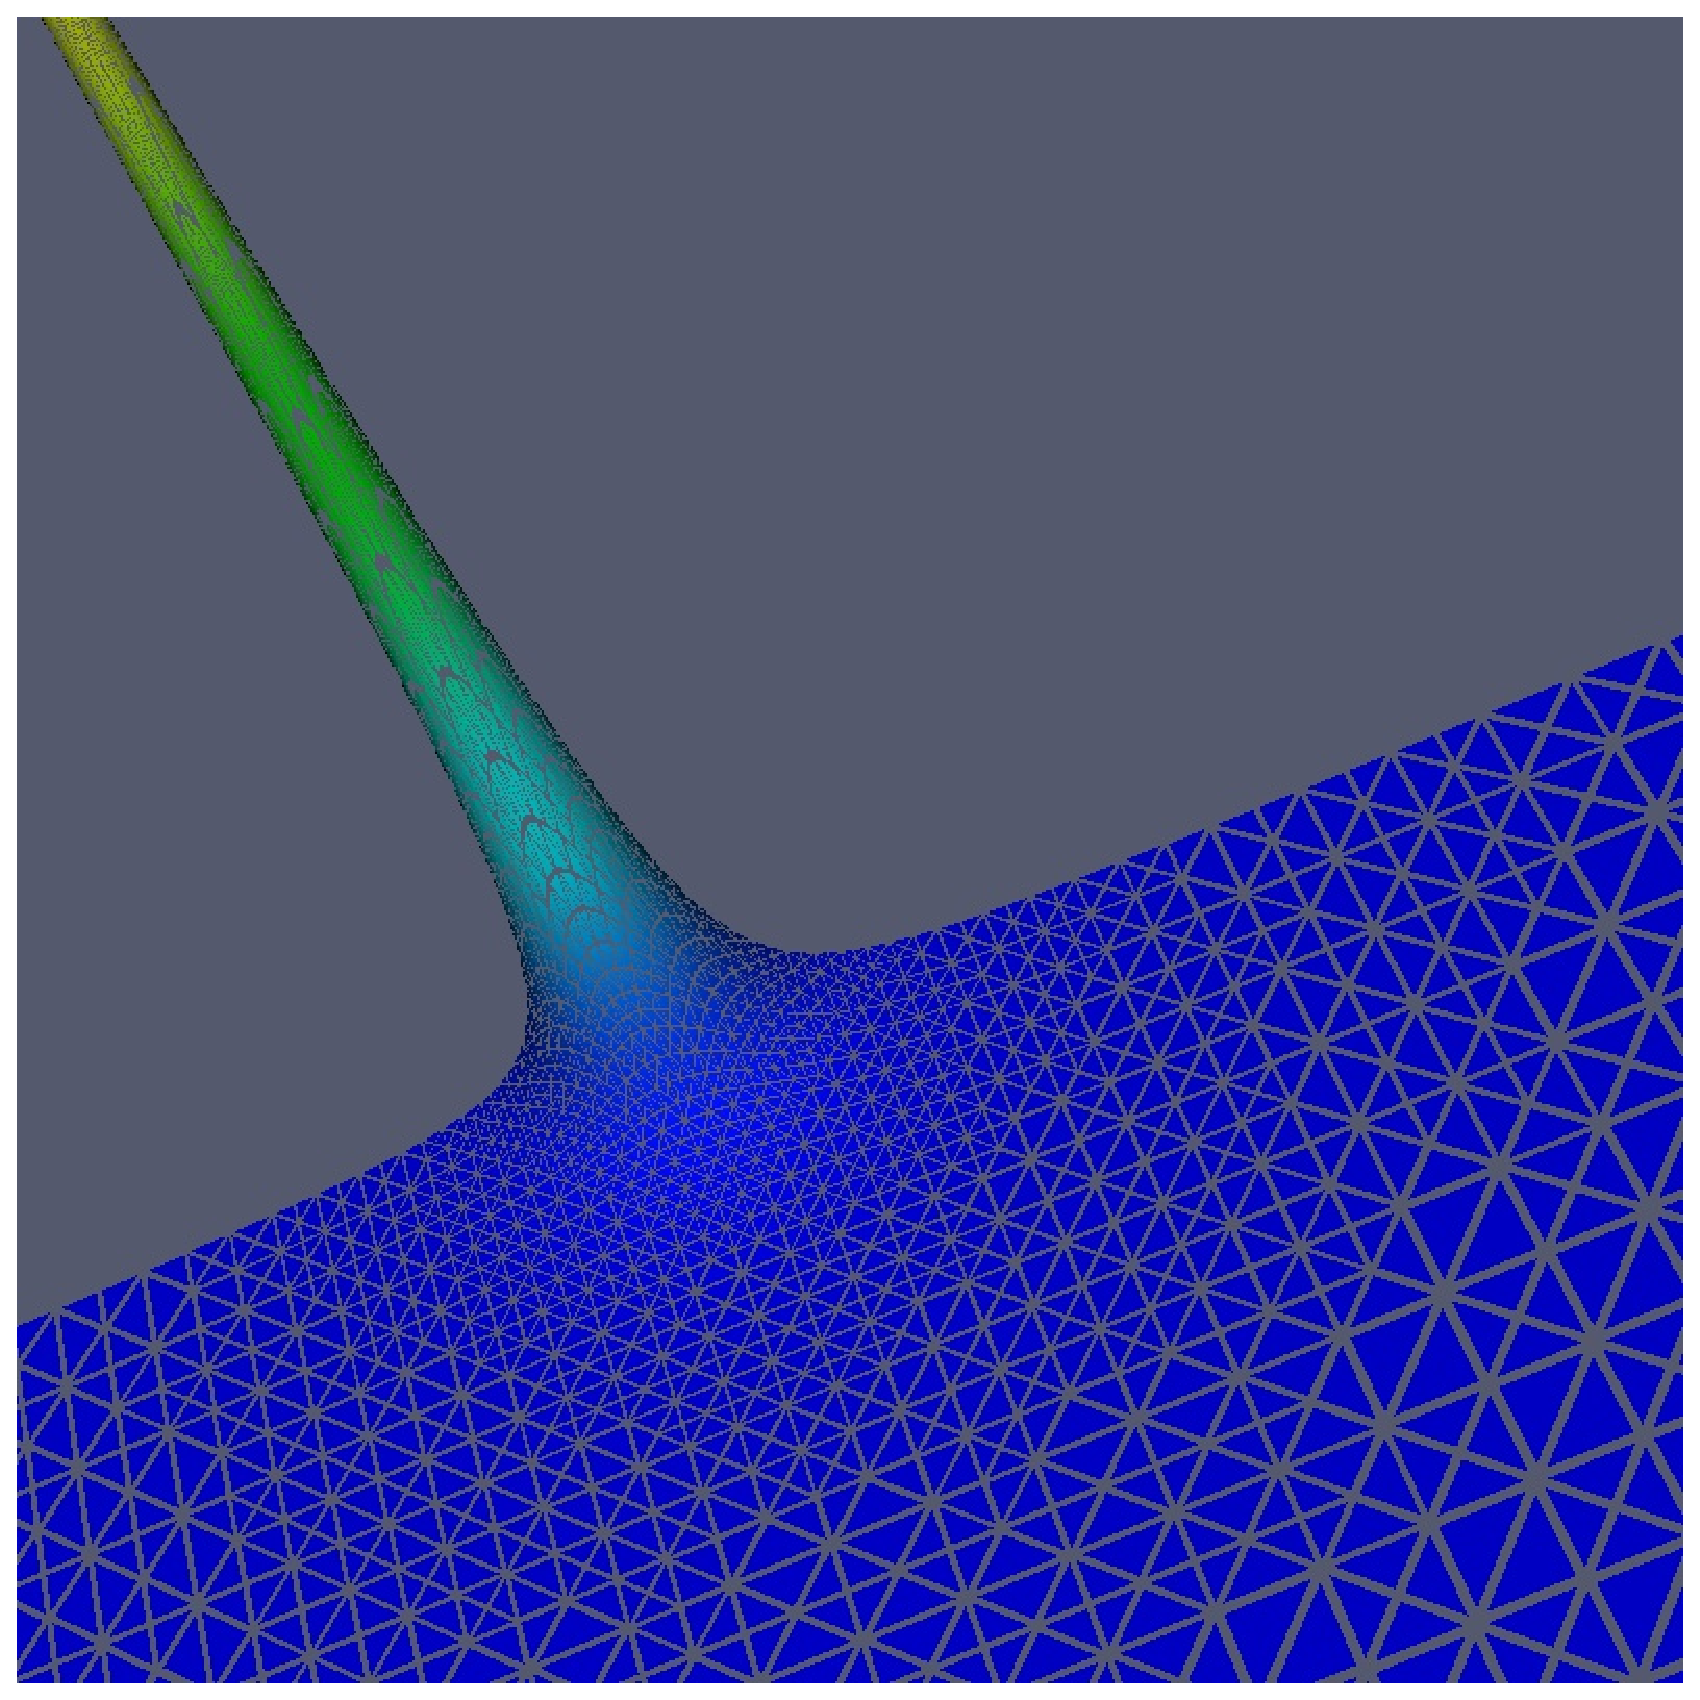
\includegraphics[width=0.48\textwidth]{EPS/adaptiveintegration_alberta2d.eps}\hfill
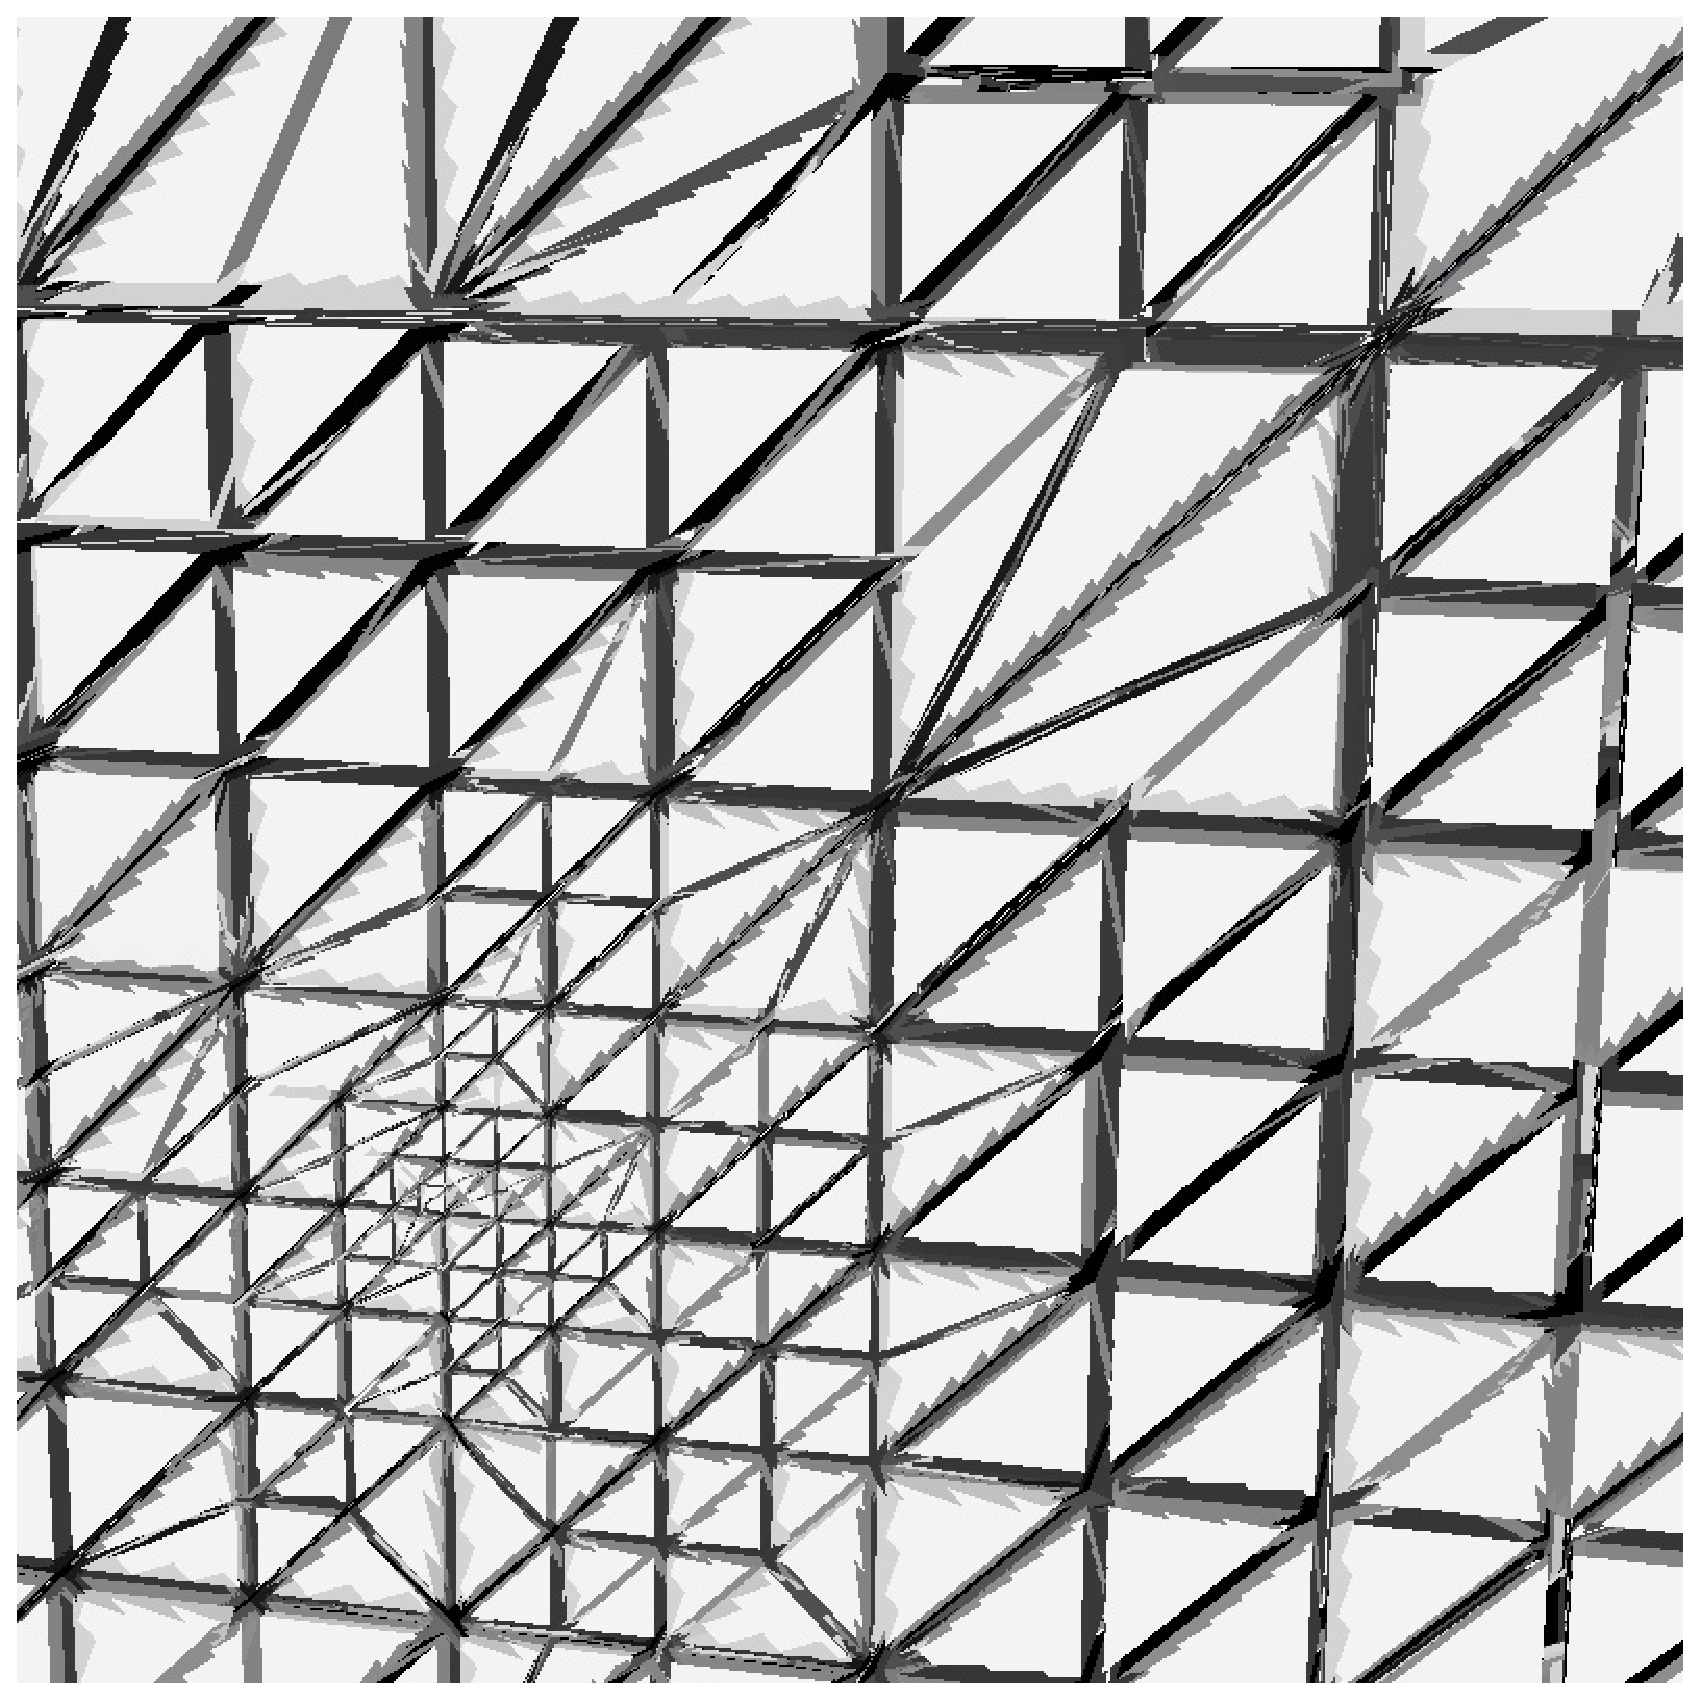
\includegraphics[width=0.48\textwidth]{EPS/adaptiveintegration_ug3d.eps}
\label{Fig:AdaptiveIntegration}
\caption{Two and three-dimensional grids generated by the adaptive
  integration algorithm applied to the needle pulse. Left grid is
  generated using Alberta, right grid is generated using UG.}
\end{figure}

Figure \ref{Fig:AdaptiveIntegration} shows two grids generated by the
adaptive integration algorithm. 

\begin{warn} The quadrature rules for prisms and pyramids are
  currently only implemented for order two. Therefore adaptive
  calculations with UGGrid and hexahedral elements do not work.
\end{warn}

\section{Cell centered finite volumes}

\begin{lst}[File dune-grid-howto/transportproblem.hh] \mbox{}
\nopagebreak
\lstinputlisting[basicstyle=\ttfamily\scriptsize,numbers=left, 
numberstyle=\tiny, numbersep=5pt]{../transportproblem.hh}
\end{lst}

\begin{lst}[File dune-grid-howto/initialize.hh] \mbox{}
\nopagebreak
\lstinputlisting[basicstyle=\ttfamily\scriptsize,numbers=left, 
numberstyle=\tiny, numbersep=5pt]{../initialize.hh}
\end{lst}

\begin{lst}[File dune-grid-howto/evolve.hh] \mbox{}
\nopagebreak
\lstinputlisting[basicstyle=\ttfamily\scriptsize,numbers=left, 
numberstyle=\tiny, numbersep=5pt]{../evolve.hh}
\end{lst}

\begin{lst}[File dune-grid-howto/vtkout.hh] \mbox{}
\nopagebreak
\lstinputlisting[basicstyle=\ttfamily\scriptsize,numbers=left, 
numberstyle=\tiny, numbersep=5pt]{../vtkout.hh}
\end{lst}

\begin{lst}[File dune-grid-howto/finitevolume.cc] \mbox{}
\nopagebreak
\lstinputlisting[basicstyle=\ttfamily\scriptsize,numbers=left, 
numberstyle=\tiny, numbersep=5pt]{../finitevolume.cc}
\end{lst}

\section{Adaptive cell centered finite volumes}

\begin{lst}[File dune-grid-howto/finitevolumeadapt.hh] \mbox{}
\nopagebreak
\lstinputlisting[basicstyle=\ttfamily\scriptsize,numbers=left, 
numberstyle=\tiny, numbersep=5pt]{../finitevolumeadapt.hh}
\end{lst}


\chapter{Parallelism}


\begin{lst}[File dune-grid-howto/parfinitevolume.cc] \mbox{}
\nopagebreak
\lstinputlisting[basicstyle=\ttfamily\scriptsize,numbers=left, 
numberstyle=\tiny, numbersep=5pt]{../parfinitevolume.cc}
\end{lst}

\begin{lst}[File dune-grid-howto/parevolve.hh] \mbox{}
\nopagebreak
\lstinputlisting[basicstyle=\ttfamily\scriptsize,numbers=left, 
numberstyle=\tiny, numbersep=5pt]{../parevolve.hh}
\end{lst}

\begin{lst}[File dune-grid-howto/parfvdatahandle.hh] \mbox{}
\nopagebreak
\lstinputlisting[basicstyle=\ttfamily\scriptsize,numbers=left, 
numberstyle=\tiny, numbersep=5pt]{../parfvdatahandle.hh}
\end{lst}

\chapter{Input and Output}

\section{Visualization with Grape}

\section{Visualization with VTK}

\section{Dune portable grid format}


\chapter{Iterative Solver Template Library}

\begin{lst}[File dune-grid-howto/groundwater.cc] \mbox{}
\nopagebreak
\lstinputlisting[basicstyle=\ttfamily\scriptsize,numbers=left, 
numberstyle=\tiny, numbersep=5pt]{../groundwater.cc}
\end{lst}

\begin{lst}[File dune-grid-howto/groundwaterproblem.hh] \mbox{}
\nopagebreak
\lstinputlisting[basicstyle=\ttfamily\scriptsize,numbers=left, 
numberstyle=\tiny, numbersep=5pt]{../groundwaterproblem.hh}
\end{lst}

\begin{lst}[File dune-grid-howto/groundwateradapt.hh] \mbox{}
\nopagebreak
\lstinputlisting[basicstyle=\ttfamily\scriptsize,numbers=left, 
numberstyle=\tiny, numbersep=5pt]{../groundwateradapt.hh}
\end{lst}






\bibliographystyle{plain}
\bibliography{grid-howto.bib}

\printindex

\end{document}
